\chapter{Case: Verified Koopa Troopa Movement}
\label{ch:case-koopa}


\section{Inleiding}

Deze eerste gevalstudie is geïnspireerd door de populaire Mario \ref{mario}
franchise van Nintendo \ref{nintendo}, in het bijzonder Super Mario Bros.
\ref{supmario}. Er zijn verschillende vijanden in het spel maar hier beperken
we ons tot de schildpadachtige Koopa Troopas. Zoals wel vaker voorkomt bevatten
vele van de Mariospellen zogenaamde \emph{glitches}, fouten die uitgebuit
kunnen worden om bepaalde acties uit te voeren die normaal moeilijk of
onmogelijk zijn. Zo is er bijvoorbeeld een fout met een Koopa Troopa waardoor
Mario aan het einde van het level over de vlag kan springen, dit is normaal
niet mogelijk. De precieze fout is moeilijk uit te leggen maar ze is mogelijk
omdat een Koopa Troopa als het ware onder het level kan rondlopen, dit is in
figuur \ref{koopaglitch} te zien. Deze fout is eigenlijk de precieze inspiratie
van deze gevalstudie.

\begin{figure}
  \centering
  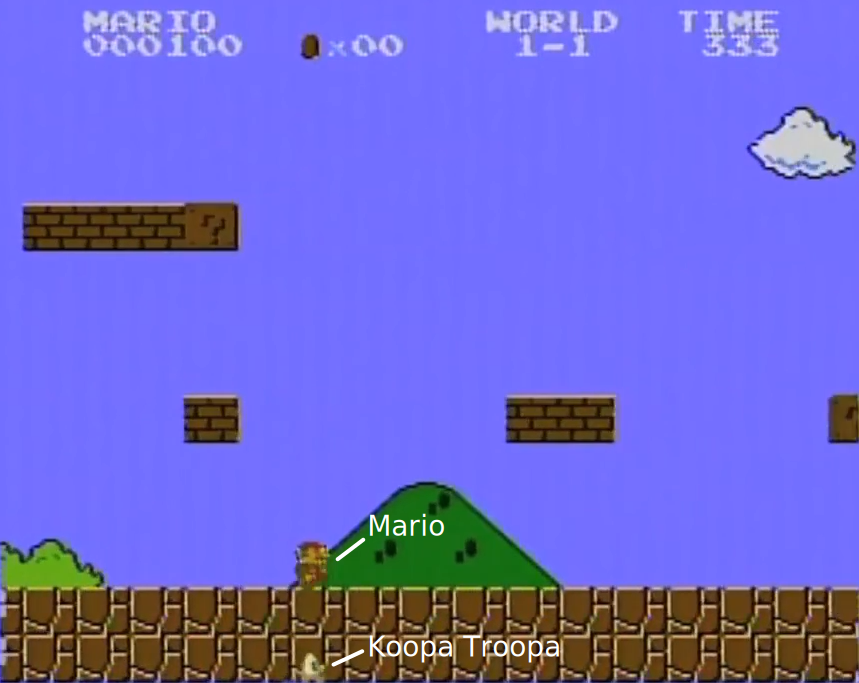
\includegraphics[width=\linewidth]{figures/KoopaTroopaGlitch}
  \caption{Onder Mario is nog net het hoofd van een Koopa Troopa te zien
           \ref{marioglitchyoutube}}
  \label{koopaglitch}
\end{figure}

De Koopa Troopas komen voor in twee kleuren: rood en groen. Ze lopen in één
richting tot ze een obstakel tegenkomen, dan keren ze om. Voor alle Koopa
Troopas is een muur een obstakel, enkel voor de rode Koopa Troopas is een
afgrond een obstakel. Dit heeft tot gevolg dat rode Koopa Troopas heen en weer
patrouilleren en groene Koopa Troopas eerder trapsgewijs naar beneden vallen
tot ze uit het beeld verdwijnen. Door deze regels uit te drukken in de types,
in plaats van in de spellogica, kunnen we een fout zoals die in figuur
\ref{koopaglitch} te zien is, voorkomen. In figuur \ref{kooparedgreen} zijn een
aantal voorbeeldpaden geïllustreerd.

\begin{figure}
  \centering
  \begin{subfigure}{0.49\textwidth}
    \includegraphics[width=\textwidth]{figures/koopatroopa-red}
  \end{subfigure}
  \begin{subfigure}{0.49\textwidth}
    \includegraphics[width=\textwidth]{figures/koopatroopa-green}
  \end{subfigure}
  \caption{Mogelijke paden voor rode en groene Koopa Troopas}
  \label{kooparedgreen}
\end{figure}


\section{Koopa Troopas in Agda}

Om het programmeren met dependent types zo duidelijk mogelijk te illustreren
wordt alle code stap voor stap bekeken in begrijpelijke stukken.  

De code begint met een module declaratie, deze is niet verplicht maar wel
nuttig omdat ze het mogelijk maakt de code te gebruiken in andere programma's.
Daarna importeren we een aantal eenvoudige types uit de standaard bibliotheek.

\inputagda[firstline=8, lastline=15, breaklines]{agda-casestt/koopa.agda}

\iagda{Data.Nat} bevat een unaire voorstelling van natuurlijke getallen die we
gaan gebruiken voor coördinaten. \iagda{Data.Fin} definieert een type voor
begrensde natuurlijke getallen, dit gebruiken we zodat we bij index operaties
niet buiten het bereik van een lijst kunnen gaan. \iagda{Data.Vec} definieert
lijsten met een vaste lengte, vectors dus. \iagda{Data.Unit} definieert een
type, \iagda{⊤} ook wel top genoemd, met één waarde namelijk \iagda{tt}. En,
ten laatste, \iagda{Data.Empty} definieert een leeg type, \iagda{⊥} ook wel
bottom genoemd, waarvoor dus geen waarden bestaan. Dit is anders dan in Haskell
waar je eigenlijk geen leeg type kunt hebben, elk type bevat daar minstens
bottom, wat verschillende dingen kan betekenen, bijvoorbeeld niet eindiging of
een error.

Het volgende stuk is een geneste module declaratie waarin het type
\iagda{Matrix} wordt gedefinieerd als een vector van vectoren en een functie
die een element uit een \iagda{Matrix} projecteert. \iagda{Matrix} is een
inductive family zoals eerder besproken. Omdat \iagda{Matrix} hier gedefinieerd
is als een vector van vectoren kunnen we voor de \iagda{lookup} functie de
\iagda{lookup} functies voor vectoren gebruiken. De volgorde van de indices
speelt hierbij een rol maar omdat de indices van het type \iagda{Fin n}
zijn, kan Agda een fout geven als we ze omwisselen. Vervolgens wordt de module
geopend zodat we het type en de functie kunnen gebruiken zonder de namen te
moeten kwalificeren met de naam van de module.

\inputagda[firstline=17, lastline=23, breaklines]{agda-casestt/koopa.agda}

Hierna begint de oplossing van het probleem eigenlijk pas echt. We definiëren
een aantal types waarmee we de Koopa Troopas en de levels kunnen voorstellen.

\inputagda[firstline=25, lastline=30, breaklines]{agda-casestt/koopa.agda}

Koopa Troopas kunnen twee kleuren hebben dus we definiëren een type
\iagda{Color} met een constructor voor elke kleur. Agda laat ons toe om
constructors met hetzelfde type te groeperen als volgt: \iagda{Green Red :
Color}. Het type \iagda{KoopaTroopa} is geïndexeerd op \iagda{Color}, dit wil
dus zeggen dat er een type is voor elke \iagda{Color}. De Constructor maakt
gebruik van de Agda syntax voor mixfix notatie, in dit geval is \iagda{KT} dus
een postfix constructor. De \iagda{_KT} constructor verwacht een
\iagda{Color} en maakt dan een waarde van het type \iagda{KoopaTroopa c} waar
die \iagda{c} dus de waarde van het argument is. Een groene Koopa Troopa kunnen
we dus voorstellen als \iagda{Green KT} en heeft het type \iagda{KoopaTroopa
Green}, later wordt duidelijk waarom het belangrijk is dat de kleur in het type
zit.

Het volgende stuk bevat nog een aantal type declaraties. Hier definiëren we
posities met alle informatie die we later nodig hebben om te bepalen op welke
posities een Koopa Troopa mag staan.

\inputagda[firstline=32, lastline=48, breaklines]{agda-casestt/koopa.agda}

Elke positie is ofwel lucht ofwel vast: grond of muur of iets dergelijks. Het
type \iagda{Material} stelt deze toestanden voor. Het type \iagda{Clearance}
gebruiken we om te bepalen wie of wat waar mag komen. Een positie met
\iagda{Clearance} \iagda{Low} kan door eender welke Koopa Troopa betreden
worden maar een positie met \iagda{Clearance} \iagda{High} kan enkel door
groene Koopa Troopas betreden worden en gebruiken we om posities aan te duiden
waar de enige logische beweging vallen is. De \iagda{Clearance}
\iagda{Ultimate} gebruiken we voor posities waar geen enkele Koopa Troopa mag
komen. Een positie stellen we voor door een record met twee velden voor een
horizontale en een verticale coördinaat, een veld dat het \iagda{Material} van
de positie aangeeft en een veld voor de \iagda{Clearance}. De constructor
\iagda{pos} kunnen we gebruiken om een positie op te stellen, een voorbeeld van
een positie kan dus zijn: \iagda{pos 3 5 gas Low}, let hierbij op dat de
cijfers door Agda begrepen worden als natuurlijke getallen, hiermee kunnen we
ook enkel natuurlijke getallen voorstellen.

Om de Koopa Troopas een \iagda{Clearance} te geven moeten we ze op een of
andere manier differentiëren en het enige dat verschilt tussen de Koopa Troopas
is hun kleur wat dus de meest logische bepalende factor van de
\iagda{Clearance} wordt.

\inputagda[firstline=50, lastline=52, breaklines]{agda-casestt/koopa.agda}

In plaats van groen en rood gelijk te stellen aan respectievelijk een hoge en
een lage \iagda{Clearance}, werkt de constructor \iagda{<red>} voor beide
kleuren terwijl \iagda{<green>} enkel voor groen werkt. Dit zorgt ervoor dat we
later niet moeten zorgen dat overal waar een lage \iagda{Clearance} toegelaten
is ook een hoge \iagda{Clearance} toegelaten is, een groene Koopa Troopa krijgt
gewoon de \iagda{Clearance} die hij nodig heeft. We zien hier ook dat de mixfix
notatie even goed voor types te gebruiken is, in dit geval gebruiken we dit om
het type voor te stellen als een pijl, \iagda{_c>_}, van een kleur naar een
\iagda{Clearance}.

De volgende twee definities zijn eigenlijk het belangrijkste deel van de
oplossing en steunen op alle voorgaande concepten.

\inputagda[firstline=54, lastline=61, breaklines]{agda-casestt/koopa.agda}

Het \iagda{_follows_⟨_⟩} type is op het eerste zicht waarschijnlijk een beetje
vreemd, dit is omdat de waarden van het type eigenlijk minder belangrijk zijn
dan het type zelf. Het type drukt uit welke positie kan volgen op welke positie
rekening houdend met een kleur. Omdat hier de types van de constructors
belangrijk zijn, overlopen we ze een voor een. \iagda{stay} drukt uit dat een
Koopa Troopa altijd kan blijven staan zolang hij in lucht staat met een lage
\iagda{Clearance}. De \iagda{Material} moet \iagda{gas} zijn omdat een Koopa
Troopa niet in grond of muren mag staan en de \iagda{Clearance} moet
\iagda{Low} zijn omdat we willen dat ook rode Koopa Troopas kunnen stilstaan.
Eigenlijk is stilstaan niet echt een nodige \emph{beweging} maar hiermee kunnen
we later de eindpositie van een pad expliciet maken. De volgende twee
constructors \iagda{next} en \iagda{back} bekijken we tegelijk omdat ze heel
gelijkaardig zijn. Ze drukken uit dat een positie met een bepaalde
\iagda{Clearance} enkel kan volgen op een horizontaal vorige, respectievelijk
volgende, positie als de kleur van de Koopa Troopa die \iagda{Clearance}
oplevert. Ook moet de voorgaande positie een lage \iagda{Clearance} hebben, dit
is omdat we de hoge \iagda{Clearance} gebruiken voor posities waar de enige
mogelijke beweging vallen is. Het \iagda{Material} voor de posities moet nog
steeds \iagda{gas} zijn omdat Koopa Troopas niet in muren kunnen lopen.  De
laatste constructor is \iagda{fall} en die kan enkel gebruikt worden als
beweging van een positie met een hoge \iagda{Clearance}. Aangezien enkel groene
Koopa Troopas op een positie met een hoge \iagda{Clearance} kunnen geraken,
zijn dat ook de enige die kunnen vallen. Nogmaals kunnen we alleen vallen van
een positie in lucht naar een positie in lucht, Koopa Troopas kunnen dus niet
de grond in vallen.

\inputagda[firstline=64, lastline=69, breaklines]{agda-casestt/koopa.agda}

Het type waarmee we de paden voorstellen die Koopa Troopas kunnen afleggen,
\iagda{Path}, moet ervoor zorgen dat enkel geldige paden worden opgesteld voor
een bepaalde Koopa Troopa. De parameter voor de kleur is impliciet omdat die
volgt uit het type van de Koopa Troopa, verder hangt de geldigheid van een pad
af van de Koopa Troopa en kan een pad maar voor één Koopa Troopa tegelijk
opgesteld worden dus is er een parameter waar we een Koopa Troopa verwachten.
Een pad gaat van een beginpositie naar een eindpositie en die moeten kunnen
variëren voor de verschillende constructors dus dat zijn indices. De
constructor voor een leeg pad, \iagda{[]}, moet een begin- en een eindpositie
hebben maar die kunnen we impliciet verkrijgen uit de vorige positie van het
pad en als er geen vorige positie is uit het verwachte type op de plaats waar
we de constructor gebruiken. De constructor om langere paden op te stellen
maakt weer gebruik van mixfix notatie, de \iagda{infixr} declaratie zorgt
ervoor dat de constructor rechts associatief is waardoor we minder haakjes
zullen nodig hebben. De constructor verwacht een positie \iagda{p}, een pad van
\iagda{q} naar \iagda{r}, \iagda{qs}, en een bewijs dat \iagda{q} kan volgen op
\iagda{p} voor de kleur van de Koopa Troopa en resulteert in een pad van
\iagda{p} naar \iagda{r}. \iagda{_↠⟨_⟩_} behoudt de geldigheid van een pad door
het argument van het type \iagda{_follows_⟨_⟩} en de enige manier om een pad te
beginnen is met een leeg pad dat sowieso geldig is. Door deze eigenschappen
zijn alle paden geldig bij wijze van constructie.

We kunnen nu paden beginnen opstellen maar een belangrijk probleem is nog dat
de geldigheid van de paden afhangt van een goede bepaling van de
\iagda{Clearance} van elke positie. Wat volgt is eerst een klein voorbeeld van
een pad en daarna een mogelijke oplossing voor een juiste bepaling van de
\iagda{Clearance} voor elke positie.

\inputagda[firstline=71, lastline=74, breaklines]{agda-casestt/koopa.agda}

Om ervoor te zorgen dat de \iagda{Clearance} juist bepaald wordt, gaan we
een functie gebruiken die de regels voor de bepaling van de \iagda{Clearance}
van een positie uitdrukt.

\inputagda[firstline=78, lastline=86, breaklines]{agda-casestt/koopa.agda}

De \iagda{matterToPosVec} functie verwacht twee vectoren van dezelfde lengte
met \iagda{Material}s in en twee coördinaten die aangeven bij welke positie het
eerste \iagda{Material} in de eerste vector hoort. Het resultaat is een vector
van dezelfde lengte met posities in met de juiste coördinaten, de
\iagda{Material}s uit de eerste vector en de juiste \iagda{Clearance} die
afhangt van het \iagda{Material} van de positie onder een positie, vandaar dat
we twee vectoren in de invoer nodig hebben. Het basisgeval is wanneer de
vectoren leeg zijn, in het andere geval bepaalt de functie \iagda{clearance}
wat de juiste \iagda{Clearance} voor de positie is aan de hand van het
\iagda{Material} van de positie zelf en van de positie er onder. Lucht boven
lucht heeft \iagda{Clearance} \iagda{High} omdat daar alleen gevallen kan
worden, lucht boven grond heeft \iagda{Clearance} \iagda{Low} omdat elke Koopa
Troopa moet kunnen staan. Alle grond en muur posities hebben \iagda{Clearance}
\iagda{Ultimate} omdat geen enkele Koopa Troopa zich in een muur of in de grond
mag bevinden.

Door vectoren te geven van alle \iagda{Material}s op een horizontale rij en de
rij daaronder kunnen we nu de \iagda{Clearance}s juist bepalen. Voor de
voorstelling van een level kunnen we dus een vector van zulke vectoren
gebruiken. Uiteindelijk willen we een matrix van posities die het level
voorstelt maar omdat het voor de recursie beter uitkomt als we met een vector
van vectoren werken voor de invoer, gebruiken we geen matrix voor de invoer.

\inputagda[firstline=88, lastline=98, breaklines]{agda-casestt/koopa.agda}

De functie \iagda{matterToPosVecs} maakt gebruik van de vorige functie om een
vector van vectoren van \iagda{Material}s om te zetten in een vector van
vectoren van posities. Het basisgeval is de lege vector en die wordt omgezet in
een lege vector. In het recursieve geval zien we dat de \iagda{_∷_} constructor
voor vectoren gebruikt wordt in de prefix vorm, dit is omdat we willen pattern
matchen op een derde impliciet argument en drie argumenten gaan niet goed samen
met een binaire infix constructor. We gebruiken \iagda{matterToPosVec} op de
eerste vector in de vector van vectoren en op de vector daaronder, die we
verkrijgen uit de functie \iagda{unders}. \iagda{unders} is eigenlijk heel
gelijkaardig aan de \iagda{head} functie maar is specifieker voor een vector
van vectoren en heeft een \emph{fallback} argument dat we teruggeven als we de
rij onder de laatste rij nodig hebben. Het enige dat dan nog rest is om de
recursieve oproep te doen op de rest van de vector van vectoren. De
\iagda{matsToMat} functie maakt van de vector van vectoren van posities, die we
terugkrijgen uit \iagda{matterToPosVecs}, een matrix waarbij de rijen eerst van
volgorde gewisseld worden omdat de index $(0,0)$ bij een matrix linksboven zit
en in de levelvoorstelling links onder.

Met deze functies kunnen we gemakkelijk een level opstellen door de juiste
\iagda{Material}s in de juiste volgorde op te geven, hierbij wordt dan meteen
de juiste \iagda{Clearance} bepaalt voor elke positie. Om onze notatie iets
visueler te maken definiëren we nog twee functies met een unicode symbool.

\inputagda[firstline=100, lastline=114, breaklines]{agda-casestt/koopa.agda}

De functies \iagda{□_} en \iagda{■_} zijn gewoon afkortingen voor
respectievelijk een vector die begint met \iagda{gas} en nog een staart
verwacht en een vector die begint met \iagda{solid} en nog een staart verwacht.
Deze functies zijn gedefinieerd met een underscore ook al zijn ze gewoon prefix
functies omdat de \iagda{infixr} declaratie enkel van toepassing is op mixfix
functies. Zoals we kunnen zien is het level, dat tevens in figuur
\ref{kooparedgreen} te zien is, redelijk herkenbaar ook al stellen we het
gewoon voor met tekst, dit is een voordeel van werken met de volledige unicode
karakterset.

Het enige dat ons nu nog rest te definiëren zijn een aantal hulp functies om
natuurlijke getallen om te zetten in getallen van het type \iagda{Fin n} omdat
we die niet met cijfers kunnen schrijven.

\inputagda[firstline=116, lastline=130, breaklines]{agda-casestt/koopa.agda}

De eerste functie, \iagda{_<'_}, vergelijkt twee natuurlijke getallen en geeft
een type terug, in een taal waar types geen waarden zijn gaat dit meestal niet.
Als het eerste getal strikt kleiner is dan het tweede is dit type \iagda{⊤},
anders is het type \iagda{⊥}. Een element van het type \iagda{⊤} kan altijd
impliciet ingevuld worden, er is er namelijk maar één: \iagda{tt}. Een element
van het type \iagda{⊥} kan nooit gegeven worden want er zijn er geen.
Van deze functie maken we gebruik in het type van \iagda{fromNat}, een functie
die een natuurlijk getal omzet in een element van \iagda{Fin n}. We kunnen een
natuurlijk getal \iagda{k} maar omzetten in een \iagda{Fin n} als \iagda{k}
strikt kleiner is dan \iagda{n}. Het type \iagda{k <' n} is ofwel gelijk aan
het type \iagda{⊤} ofwel aan het type \iagda{⊥}, in het eerste geval moeten we
dus geen expliciete waarde geven, in het tweede geval kunnen we geen waarde
geven en dus kunnen we de functie ook niet oproepen met een \iagda{k} die we
nooit kunnen omzetten in een \iagda{Fin n}. Op deze manier kan de typechecker
ons waarschuwen wanneer we dit ergens wel proberen doen. In deze functie zien
we nog iets nieuws, de eerste vergelijking heeft geen rechterzijde. Dit is
omdat er geen waarde bestaan van het type \iagda{Fin n}, dat isomorf is met het
type \iagda{⊥}. Omdat de \iagda{n} in \iagda{Fin n} een natuurlijk getal is, is
\iagda{0} niet uitgesloten en omdat Agda een totale programmeertaal is moeten
we voor elke mogelijke waarde van het argument \iagda{n} een antwoord bieden.
In dit geval is het type \iagda{k <' n} sowieso gelijk aan \iagda{⊥} en omdat
we geen waarde van dat type kunnen krijgen kunnen we gebruik maken van het
zogenaamde \emph{absurd} pattern: \iagda{{}} of \iagda{()}. Het absurd pattern
geeft aan dat er onmogelijk een waarde van het juiste type bestaat, de
typechecker moet dit wel kunnen nagaan dus dit werkt alleen voor types die
eenvoudig genoeg zijn. Als Agda overtuigd is dat er geen waarde bestaat, moeten
we ook geen rechterzijde opgeven. In de derde vergelijking zien we nog dat het
\emph{bewijs} dat \iagda{k} kleiner is dan \iagda{n} expliciet doorgegeven
wordt en dus geldig blijft voor het recursieve geval, het is tenslotte ook maar
een eenvoudige waarde, \iagda{tt}. De functie \iagda{f} is slechts een
afkorting voor \iagda{fromNat}. De functie \iagda{p} is een afkorting voor
\iagda{lookup} waarbij de coördinaten omgewisseld zijn voor de leesbaarheid en
het level niet moet opgegeven worden omdat dat in alle voorbeelden hetzelfde
is.

Met al deze extra definities kunnen we nu paden op een compacte manier
definiëren zoals we in de rest van de voorbeelden zien.

\inputagda[firstline=132, lastline=144, breaklines]{agda-casestt/koopa.agda}

\iagda{red_path_one} en \iagda{red_path_two} stellen de paden voor die door de
rode Koopa Troopas afgelegd wordt in figuur \ref{kooparedgreen}, het vakje
linksonder heeft coördinaat $(0,0)$, de x-as loopt horizontaal en de y-as
verticaal. Voorbeelden van paden waar niets mis mee is zijn eigenlijk niet zo
interessant, die kunnen in het originele spel ook voorgesteld worden. Het wordt
pas interessant als we proberen om een ongeldig pad op te stellen want dat is
wat we proberen te voorkomen.

\inputagda[firstline=1, lastline=12, breaklines]{agda-casestt/koopa-errors.agda}

De fout bij \iagda{red_nopath_one} ziet eruit als volgt:

%----------------------------------------%
\begin{minted}[fontsize=\small]{agda}
  gas != solid of type Material
  when checking that the expression stay has type
  pos 0 (suc zero) gas Low follows p (f 0) (f 1) ⟨ Red ⟩
\end{minted}

Agda geeft aan dat de positie in het type van \iagda{stay} niet overeenkomt met
de positie, door \iagda{stay} te gebruiken op positie $(0,1)$ zou het type
\iagda{pos 0 1 solid Ultimate follows pos 0 1 solid Ultimate ⟨ Red ⟩} moeten
zijn maar dat is niet toegelaten in de definitie van de constructor.
Eigenlijk verwachten we een fout daar waar we een muur in lopen en hier krijgen
we de fout pas te zien als we al in een muur staan. Dit is omdat de
\iagda{_↠⟨_⟩_} constructor rechts associatief is, dus de eerste fout die Agda
tegenkomt zit zo ver mogelijk vanachter in het pad.

In de fout voor \iagda{red_nopath_two} kunnen we zien dat de beweging waarbij
we een muur zouden inlopen wel als fout wordt gezien:

%----------------------------------------%
\begin{minted}[fontsize=\small]{agda}
  gas != solid of type Material
  when checking that the expression p (f 1) (f 1) ↠⟨ back ⟩ [] has
  type Path (Red KT) (p (f 1) (f 1)) (p (f 0) (f 1))
\end{minted}

Deze fout is zo goed als hetzelfde als de vorige, alleen gaat het nu om de
\iagda{back} constructor en is de expressie waar de fout zich bevindt niet even
ver gereduceerd omdat het type van \iagda{back} ingewikkelder is.

Een pad voor een rode Koopa Troopa moet ook ongeldig zijn als een Koopa Troopa
zou vallen bij het afleggen van het pad:

%----------------------------------------%
\begin{minted}[fontsize=\small]{agda}
  Low != High of type Clearance
  when checking that the expression p (f 4) (f 1) ↠⟨ next ⟩ [] has
  type Path (Red KT) (p (f 4) (f 1)) (p (f 5) (f 1))
\end{minted}

Als een rode Koopa Troopa van een afgrond afloopt, is het niet het
\iagda{Material} dat in de weg zit, het is namelijk allemaal lucht, maar wel
het feit dat een rode Koopa Troopa niet de juiste \iagda{Clearance} heeft.

Voor een groene Koopa Troopa kunnen we opnieuw geldige paden opstellen:

\inputagda[firstline=159, lastline=184, breaklines]{agda-casestt/koopa.agda}

In \iagda{green_path_one} zien we één van de geldige paden voor rode Koopa
Troopas terugkomen. Een pad dat geldig is voor een rode Koopa Troopa is ook
geldig voor een groene Koopa Troopa. In het oorspronkelijke spel zijn Koopa
Troopas ook obstakels voor elkaar, op die manier zou een groene Koopa Troopa
dus beperkt kunnen worden tot een pad dat een rode ook kan afleggen. Evenzeer
is een pad voor een rode Koopa Troopa dat omkeert voor er een obstakel in de
weg zit, mogelijk. Opnieuw kan dit nuttig zijn, bijvoorbeeld om de Koopa
Troopas actief de speler te laten achtervolgen als die in de buurt komt,
waarbij ze dus vroeger dan nodig omkeren. In \iagda{green_path_two} zien we het
langere pad dat in figuur \ref{kooparedgreen} geïllustreerd is.

Voor een groen Koopa Troopa is het geen fout als het pad van een afgrond af
gaat en dan naar beneden valt. Maar er treedt zoals verwacht nog wel een fout
op als we proberen een muur in te lopen:

\inputagda[firstline=14,lastline=16,breaklines]{agda-casestt/koopa-errors.agda}

%----------------------------------------%
\begin{minted}[fontsize=\small]{agda}
  gas != solid of type Material
  when checking that the expression p (f 1) (f 1) ↠⟨ back ⟩ [] has
  type Path (Green KT) (p (f 1) (f 1)) (p (f 0) (f 1))
\end{minted}

Deze fout is identiek aan die voor \iagda{red_nopath_two}. In het volgende
deel bespreken we de implementatie van dit model in Haskell.


\section{Koopa Troopas in Haskell}

In Haskell beginnen we de code met de LANGUAGE pragma's die besproken zijn in
hoofdstuk \ref{ch:agda-haskell}. Daarna komt de module declaratie, hier zien we
voor de eerste keer dat Haskell redelijk strikte regels heeft over naamgeving,
modules types en constructors moeten met een hoofdletter beginnen en functies
met een kleine letter.

\inputhaskell[firstline=8, lastline=11, breaklines]{haskell-casestt/koopa.hs}

Om te beginnen moeten we een aantal types die we in Agda uit de standard
library kunnen halen zelf implementeren or is bijvoorbeeld geen erg grote nood
aan een unaire voorstelling van natuurlijke getallen in Haskell. De naamgeving
en technieken die we hier gebruiken komen uit een artikel \ref{hasochism} over
dependently typed programmeren in Haskell met de titel: "Hasochism: The
Pleasure and Pain of Dependently Typed Haskell Programming." Het wordt redelijk
snel duidelijk waarom het artikel die titel heeft.

\inputhaskell[firstline=13, lastline=24, breaklines]{haskell-casestt/koopa.hs}

We beginnen met het definiëren van onze unaire natuurlijke getallen, dankzij de
datatype promotion van de DataKinds extensie hebben we nu ook meteen unaire
natuurlijke getallen op het typeniveau. Wat we nog missen is een verbinding
tussen waarden op het waardeniveau en waarden op het typeniveau zoals die er
wel is in Agda, daar kunnen we een argument van de functie ook in het type
gebruiken. In Haskell kunnen we dit niet echt doen maar we kunnen het wel
imiteren met een zogenaamde singleton constructie. Dit zien we in de definitie
van \ihask{Natty n}, elke waarde die we opstellen heeft een ander type:
\ihask{Zy} heeft type \ihask{Natty Z} en \ihask{Sy Zy} heeft type \ihask{Natty
(S Z)}. Omdat elk type \ihask{Natty n} maar één waarde bevat, heeft deze
constructie de benaming singleton gekregen. De functie \ihask{natter}, ongeveer
te lezen als "meer Nat-achtig," zet een \ihask{Natty n} om in een \ihask{Nat},
hierbij werpen we als het ware informatie op het typeniveau weg. De omgekeerde
conversie gaat niet zomaar, er is geen manier om statisch te bepalen wat de
\ihask{n} in het return type \ihask{Natty n} zou moeten zijn. Om dit bij
benadering toch te kunnen doen hebben we een derde type nodig, \ihask{NATTY}.
Dit type verstopt als het ware de typeniveau informatie van een \ihask{Natty
n}. Nu kunnen we de functie \ihask{nattyer}, "meer Natty-achtig," wel
schrijven. De definitie is eenvoudig, in het recursieve geval moeten we een
pattern match doen op de recursieve oproep om met de eigenlijke waarde van de
\ihask{Natty n} te kunnen werken.

Haskell ontbreekt logischerwijs tevens een type voor begrensde natuurlijke
getallen. Deze keer kunnen we de extra types niet definiëren omdat Haskell het
\ihask{Fin n} type niet kan promoveren. De DataKinds extensie promoveert enkel
types met argumenten met kind \ihask{*}.

\inputhaskell[firstline=27, lastline=35, breaklines]{haskell-casestt/koopa.hs}

De definitie voor \ihask{Fin n} is identiek aan die uit de Agda standard
library voor zover dat mogelijk is. De functie \ihask{intToFin} dient ongeveer
hetzelfde doel als de \iagda{fromNat} functie uit de Agda code. Omdat Haskell
geen cijfers toelaat voor natuurlijke getallen, vertrekken we van het
\ihask{Integer} type. Dit brengt met zich mee dat we negatieve getallen
toelaten, hiervoor werpen we gewoon een fout op.

Vervolgens is er het type \ihask{Vec} dat ook weer logischerwijs niet in
Haskell aanwezig is met de bijhorende functies.

\inputhaskell[firstline=38, lastline=58, breaklines]{haskell-casestt/koopa.hs}

Haskell laat binaire infix constructors toe door hun naam te beginnen met een
dubbelpunt, toevallig kunnen we zo bijna dezelfde notatie gebruiken als in
Agda. \ihask{vlookup} haalt een element uit een vector met behulp van een
begrensd getal dus we sluiten uit dat een index te groot of te klein is.
\ihask{vreplicate} stelt een vector op met een bepaald aantal herhalingen van
een element, we hebben hier een \ihask{Natty n} nodig omdat we de waarde
\ihask{n} moeten kennen voor het type van de vector die we willen teruggeven.
\ihask{vreverse} keert de volgorde van de elementen in een vector om.

Nu kunnen we ook het \ihask{Matrix} type definiëren. Dit type en de voorgaande
types zijn niet gedefinieerd in submodules zoals we \iagda{Matrix} gedefinieerd
hebben in Agda omdat Haskell geen concept heeft van submodules. We zouden deze
types allemaal in modules in hun eigen bestanden kunnen definiëren maar omdat
het weinig code is en slechts tot voorbeeld dient, is dit achterwege gelaten.

\inputhaskell[firstline=61, lastline=65, breaklines]{haskell-casestt/koopa.hs}

Zowel het \ihask{Matrix} type als de \ihask{mlookup} functie gelijken sterk op
hun tegenhangers in Agda. Het grootste verschil is dat we in Haskell met
polymorfisme werken daar waar we in Agda gewoonlijk impliciete argumenten
gebruiken.


